	The driver used to connect to the databases recommends to have one database connection for the entire application \cite{web:mongodb16}. In order to guarantee this requirement, we have implemented the Singleton pattern which ensures that only one instance of a class is created and provides a global access point to the database connection.

	The Figure \ref{fig:design:singletonPattern} describes the enum type DBConnection that works according to this creational pattern.

	\begin{figure}[H]
	\centering
	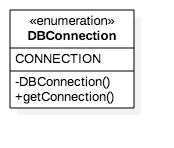
\includegraphics[max size={\textwidth}{\textheight}]{design/img/singleton.png}
	\caption{Singleton Design Pattern for the database connection}
	\label{fig:design:singletonPattern}
	\end{figure}

	The implementation that we have designed, improves the normal style followed for defining singleton objects in Java. Usually the singleton objects have to be wrapped with a synchronised declaration method in order to avoid for simultaneous clients to create multiple instances. Our singleton connector for databases follows Bloch idea that consist in declaring an enumeration type for the singleton object (e.g. CONNECTION) \cite{book:bloch08}. As the enumeration type is considered thread safe by default not only avoids the need for wrapping the object creation but also offers other interesting benefits such as serialization and reflection.

	